\section{Arhitectura demonstraţiilor de concept WT SDN}

Așa cum a fost amintit anterior, proiectul \textit{Wireless Transport} din grupul Open Transport Working Grup din cadrul \gls{onf} se ocupă cu cercetare legată de \gls{sdn} în contextul rețelelor de transport de date fără fir. După cum este prezentat și în \cite{bercovich2015software, bernardos2014architecture}, acest tip de rețele sunt o parte importantă atât din perspectiva rețelelor curente, cât și din cea a rețelelor viitorului, precum cele 5G.

După efectuarea unei demonstraţii de concept \cite{onf2015_poc1} care folosea protocolul OpenFlow pentru a arăta capabilitățile \gls{sdn} în rețelele de transport de date fără fir, observând dificultăţile pe care le presupune lucrul cu OpenFlow în acest context, grupul a trecut la dezvoltarea unui model informațional care să abstractizeze dispozitivele ce fac parte din aceste rețele, model care a fost descris anterior.

Apoi, alte trei demonstraţii de concept au avut loc, descrise în \cite{onf2016_poc2, onf2016_poc3, onf2017_poc4}, care au urmărit evoluția acestui model informațional. Chiar dacă în cel de-al doilea \gls{poc} s-a folosit un model de date mult simplificat, iar în cel de-al patrulea a fost folosită cea mai bună și matură variantă a sa, arhitectura acestor demonstraţii a fost similară.

\begin{figure}[h]
	\centering
	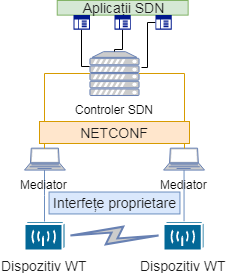
\includegraphics{poc_architecture}
	\caption{Arhitectura demonstraţiilor de concept WT.}
	\label{fig:poc_architecture}
\end{figure}

După cum se poate observa în Figura \ref{fig:poc_architecture}, în arhitectura acestor demonstraţii apare nevoia unui nivel intermediar, de mediator. Acest mediator este reprezentat de o aplicație software care expune o interfață \gls{netconf} către nord, unde se conectează echipamentul de control \gls{sdn}, folosind modelul informațional descris de TR-532. Rolul mediatorului este de a traduce comenzile \gls{netconf} care vin de la controler în comenzi pe care dispozitivul de rețea le poate înţelege (de exemplu \gls{snmp}, \gls{cli} sau \gls{rest}). Această nevoie apare din cauza faptului că echipamentele din rețelele actuale, care au fost folosite și pentru demonstraţiile de concept, nu suportă încă noul model informațional în mod nativ, deoarece abia a fost dezvoltat. Cel mai probabil, în viitor această nevoie va dispărea, echipamentele putând să încadreze \textit{Microwave Model} în aplicaţia software proprie de control.

\begin{figure}[t]
	\centering
	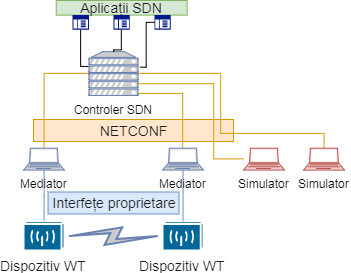
\includegraphics{poc_architecture_simulator}
	\caption{Poziţionarea simulatoarelor în arhitectura demonstraţiilor de concept WT.}
	\label{fig:poc_architecture_simulator}
\end{figure}


Poziţionarea simulatoarelor în arhitectura acestor demonstraţii de concept este ilustrată în Figura \ref{fig:poc_architecture_simulator}. Astfel, ele pot fi folosite de către dezvoltatorii de aplicații \gls{sdn} pentru testarea aplicațiilor care utilizează interfaţa \gls{netconf} ce implementează modelul informațional TR-532, eliminând nevoia acestora de a deţine dispozitive pentru transportul de date fără fir și mediatorul asociat acestora.